\documentclass[12pt]{article}
\usepackage[letterpaper, portrait, margin=1in]{geometry}
\usepackage{amsmath, amsthm, amssymb, mathrsfs, dsfont}

\usepackage{graphicx}
\graphicspath{{/Users/darshanpatel/Desktop/LaTex Notes/Math333/}}

\usepackage{fancyhdr}
\pagestyle{fancy}
\fancyhf{}
\lhead{Darshan Patel}
\rhead{Math 333: Introduction to Algebraic Structures}
\renewcommand{\footrulewidth}{0.4pt}
\cfoot{\thepage}

\newcommand{\sectionbreak}{\clearpage}

\renewcommand{\times}{\ast}
\newcommand{\inverse}[1]{#1 ^{-1}}
\newcommand{\pinverse}[1]{(#1)^{-1}}
\newcommand{\set}[1]{\{ #1 \}} 
\newcommand{\group}[2]{\langle #1, #2 \rangle}
\newcommand{\integers}{\mathds{Z}}
\newcommand{\rationals}{\mathds{Q}}
\newcommand{\nonzerorationals}{\mathds{Q}^*}
\newcommand{\nonzeroreals}{\mathds{R}^*}
\newcommand{\reals}{\mathds{R}}
\newcommand{\complex}{\mathds{C}}





\begin{document}

\theoremstyle{definition}
\newtheorem{theorem}{Theorem}[section]
\newtheorem{definition}{Definition}[section]
\newtheorem{example}{Example}[section]

\title{Math 333: Introduction to Algebraic Structures}
\author{Darshan Patel}
\date{Fall 2017}
\maketitle

\tableofcontents



\section{Operations} 
\begin{definition} Let $A$ be any set: \\ An operation $\times$ on $A$ is a rule which assigns to each ordered pair $(a, ~b)$ of elements of $A$ exactly one element $a \times b$ in $A$. \end{definition}

Stressed Aspects: \begin{itemize} 
\item $a \times b$ is defined for every ordered pair $(a, ~b)$ of elements of $A$. Often, $a \times b$ is defined for all the obvious choices of $a$ and $b$, but remains undefined in a few exceptional cases. 

\begin{example} Division does not qualify as an operation on the set $ \reals $ of the real numbers, for there are ordered pairs such as $(3, ~0)$ whose quotient $3/0$ is undefined. In order to be an operation on $\reals$, division would have to associate a real number $a/b$ with every ordered pair $(a, ~b)$ of elements of $\reals$. \end{example} 

\item $a \times b$ must be uniquely defined. 

\begin{example} Define an operation $\square$ on the set $\reals$ of the real numbers by letting $a \square b$ be the number whose square is $ab$. This is ambiguous because $2 \square 8$ could be either 4 or -4. Thus $\square$ does not qualify as an operation on $\reals$. \end{example}

\item If $a$ and $b$ are in $A$, $a \times b$ must be in $A$. This is expressed by saying that $A$ is closed under the operation $\times$. 

\begin{example} Division cannot be regarded as an operation on the set of the integers, for there are pairs of integers such as (3, 4) whose quotient $3/4$ is not an integer. \\ On the other hand, division does qualify as an operation on the set of all the positive real numbers, for the quotient of any two positive real numbers is a uniquely defined positive real number. \end{example}

\end{itemize}

An operation is any rule which assigns to each ordered pair of elements of $A$ a unique element in $A$. Therefore in general, there are many possible operations on a given set $A$. 

\begin{example} If $A$ is a set consisting of 2 distinct elements, $a$ and $b$, each operation on $A$ may be described by a table as follows 
$$ \begin{tabular}{c|c}  
$(x, y)$ & $x \times y$ \\ \hline 
$(a, a)$ \\ \hline $(a, b)$ \\ \hline $(b, a)$ \\ \hline $(b, b)$ \\  \end{tabular}$$ 
Here are four possible operations for four possible ordered pairs of elements of $A$ and the value of $x \times y$ 

$$ \begin{tabular}{c|c|c|c|c|}
$(x, y)$ & $1)~ x \times y $ & $ 2)~ x \times y $ & $ 3)~ x \times y $ & $ 4)~ x \times y $ \\ \hline 
$(a, a)$ & $a$ & $a$ & $b$ & $b$ \\ \hline 
$(a, b)$ & $a$ & $b$ & $a$ & $b$ \\ \hline 
$(b, a)$ & $a$ & $a$ & $b$ & $b$ \\ \hline 
$(b, b)$ & $a$ & $b$ & $a$ & $a$ \end{tabular}$$ 
Each row describes a different operation on $A$. In fact, there are 16 possible ways of filling the table and thus 16 possible operations on the set $A$. \end{example} 

\begin{definition} An operation $\times$ may be commutative, that is, it may satisfy $$ a \times b = b \times a$$ for any two elements $a$ and $b$ in set $A$. \end{definition}

\begin{definition} An operation $\times$ may be associative, that is, it may satisfy $$ (a \times b) \times c = a \times (b \times c) $$ for any 3 elements $a$, $b$ and $c$ in set $A$. \end{definition} 

\begin{example} The addition of real numbers is associative because $$a + (b + c) = (a + b) + c$$
However, division of real numbers is not associative $$ \frac{3}{4/5} = \frac{15}{4} \text{ but } \frac{3/4}{5} = \frac{3}{20} $$ \end{example} 

\begin{definition} If there is an element $e$ in $A$ with the property that $e \times a = a$ and $a \times e = a$ for every element $a$ in $A$, then $e$ is called an identity of ``neutral'' element with respect to the operation $\times$. When combined with any element $a$, it does not change $a$. \end{definition} 

\begin{example} In the set $\reals$ of the real numbers, 0 is a neutral element for addition and 1 is a neutral element for multiplication. \end{example} 

\begin{definition} If $a$ is any element of $A$ and $x$ is an element of $A$ such that $a \times x = e$ and $x \times a = e$, then $x$ is called an inverse of $a$. When an element is combined with its inverse, it produces the neutral element. \end{definition} 

\begin{example} In the set $\reals$ of the real numbers, $-a$ is the inverse of $a$ with respect to addition; if $a \neq 0$, then $\frac{1}{a}$ is the inverse of $a$ with respect to multiplication. \end{example} 
Note: Usually, the inverse of $a$ is denoted by $a^{-1}$. 


\section{The Definition of Groups} 

\begin{definition} By a group, we mean a set $G$ with an operation $\times$ which satisfies the axioms: 
\begin{enumerate} 
\item $\times$ is associative 
\item There is an element $e$ in $G$ such that $a \times e = a$ and $e \times a = a$ for every element in $G$ 
\item For every element $a$ in $G$, there is an element $a^{-1}$ in $G$ such that $a \times a^{-1} = e$ and $a^{-1} \times a = e$ \end{enumerate} \end{definition}

 Note: A group is represented by the symbol $\group{G}{\times}$. 
 
 \begin{example} $\integers$ is the symbol used to denote the set $$\set{\dots, -3. -2, -1, 0, 1, 2, 3, \dots} $$ of the integers. The set $\integers$, with the operation of addition, is obviously a group. It is called the additive group of the integers and represented by the symbol $\group{\integers}{+}$. Mostly, it is denoted simply by the symbol $\integers$. \end{example} 
 
 \begin{example} $\rationals$ designates the set of the rational numbers (that is, quotients $m/n$ of integers where $n \neq 0$). This set, with the operation of addition, is called the additive group of the rational numbers, $\group{\rationals}{+}$. It is denoted by $\rationals$. \end{example} 
 
 \begin{example} The symbol $\reals$ represents the set of the real numbers. $\reals$ with the operation of addition, is called the additive group of the real numbers and is represented by $\group{\reals}{+}$, or simply $\reals$. \end{example}
 
 \begin{example} The set of the nonzero rational numbers is represented by $\nonzerorationals$. This set, with the operation of multiplication, is the group $\group{\nonzerorationals}{\cdot}$, or simply $\nonzerorationals$. \\ Similarly, the set of all the nonzero real numbers is represented by $\nonzeroreals$. The set $\nonzeroreals$ with the operation of multiplication, is group $\group{\nonzeroreals}{\cdot}$, or simply $\nonzeroreals$. \end{example} 
 
 \begin{example} $\rationals^{\text{pos}}$ denotes the group of all the positive rational numbers, with multiplication. $\reals^{\text{pos}}$ denotes the group of all the positive real numbers, with multiplication. \end{example} 
 
 \begin{definition} Finite Groups: groups with a finite number of elements \end{definition} Such groups occur often in applications, for in most situations of the real world, we deal with only a finite number of objects. 
 
 \begin{definition} Group of Integers modulo $n$: consists of the set $$\set{0, 1, 2, \dots, n - 1}$$ with the operation of addition modulo $n$. Imagine the numbers 0 through $n - 1$ to be points on the unit circle, each one separated from the next by an arc of length $2\pi / n$. To add two numbers $h$ and $k$, start with $h$ and move clockwise through an arc of $k$ times $2\pi / n$. The sum $h + k$ will be one of the numbers 0 through $n - 1$. From geometrical considerations it is clear that this kind of addition is associative. Zero is the neutral element of this group and $n - h $ is the inverse of $h$ [for $h + (n - h) = n$, which coincides with 0]. This group, the group of integers modulo $n$, is represented by the symbol $\integers_n$. \end{definition} 
 
 When working with finite groups, it is useful to draw up an ``operation table.'' The basic format of this table is as follows 
 $$\begin{tabular}{c|cccccc} + & 0 & 1 & 2 & 3 & 4 & 5 \\ \hline 
 0 \\ 1 \\ 2 \\ 3 \\ 4 \\ 5 \end{tabular} $$ 
 with one row for each element of the group and one column for each element of the group. Then, for example, 3 + 4, is located in the row of 3 and the column of 4. In general, any finite group $\group{G}{\times}$ has a table $$\begin{tabular}{c|ccc} 
$\times$ & $\cdots \cdots$ & $y$ & $\cdots \cdots$ \\ \hline 
 $\vdots$ \\ $x$ & & $x + y$ & \\ $\vdots$ \end{tabular}$$ 
 The entry in the row of $x$ and the column of $y$ is $x \times y$. \\sim\\
 Note that the commutative law is not one of the axioms of group theory; hence the identity $ a\ times b = b \times a$ is not true for every group. If the commutative law holds in a group $G$, such a group is called a commutative group, or more commonly, an abelian group. 
 
 \begin{example} Let $G$ be the group which consists of the six matrices 
 $$ I = \begin{pmatrix} 1 & 0 \\ 0 & 1 \end{pmatrix} ~~ A = \begin{pmatrix} 0 & 1 \\ 1 & 0 \end{pmatrix} ~~ B = \begin{pmatrix} 0 & 1 \\ -1 & -1 \end{pmatrix} $$
 $$C = \begin{pmatrix} -1 & -1 \\ 0 & 1 \end{pmatrix} ~~ D = \begin{pmatrix} -1 & -1 \\ 1 & 0 \end{pmatrix} ~~ K = \begin{pmatrix} 1 & 0 \\ -1 & -1 \end{pmatrix} $$ with the operation of matrix multiplication. this group has the following operation table 
 $$\begin{tabular}{c|cccccc} & 1 & A & B & C & D & K \\ \hline 
 1 & I & A & B & C & D & K \\
 A & A & I & C & B & K & D \\
 B & B & K & D & A & I & C \\ 
 C & C & D & K & I & A & B \\ 
 D & D & C & I & K & B & A \\ 
 K & K & B & A & D & C & I \end{tabular} $$ 
 In linear algebra it shown that the multiplication of matrices is associative. It is clear that $I$ is the identity element of this group and by looking at the table, one can see that each of the six matrices in $[I, A, B, C, D, K]$ has in inverse in $[I, A, B, C, D, K]$. For example, $B$ is the inverse of $D$, $A$ is the inverse of $A$, and so on. Thus $G$ is a group! Note however that $AB = C$ but $BA = K$, so $G$ is not commutative. $G$ is not an abelian group. \end{example}

\section{Elementary Properties of Groups}

Is it possible for a group to have two different identity elements? Suppose $e_1$ and $e_2$ are identity elements of some group $G$. Then $$\begin{aligned} e_1 \times e_2 &= e_2 \text{ because } e_2 \text{ is an identity element, and } \\ e_1 \times e_2 &= e_1 \text{ because } e_2 \text{ is an identity element} \end{aligned} $$ 
Therefore $$e_1 = e_2$$ This shows that in every group, there is exactly one identity element. \\sim\\

Can an element $a$ in a group have different inverses? If $a_1$ and $a_2$ are both inverses of $a$, then 
$$ a_1 \times (a \times a_2) = a_1 \times e = a_1$$ and $$(a_1 \times a) \times a_2 = e \times a_2 = a_2 $$
By the associative law, $a_1 \times (a \times a_2) = (a_1 \times a) \times a_2$. Hence $a_1 = a_2$. This shows that in every group, each element has exactly one inverse. 

\begin{definition} Additive Notation: refers $a + b$ as the sum of $a$ and $b$ \end{definition} 

\begin{definition} Multiplicative Notation: refers $ab$ as the product of $a$ and $b$ \end{definition} 

\begin{theorem} Cancellation Law: If $G$ is a group and $a$, $b$, $c$ are elements of $G$, then 
\begin{enumerate} 
\item $ab = ac$ implies $b = c$
\item $ba = ca$ implies $b = c$ \end{enumerate} \end{theorem} 

\begin{proof} Suppose $$ab = ac$$ Then $$\inverse{a}(ab) = \inverse{a}(ac) $$ 
By the associative law, $$(\inverse{a}a)b = (\inverse{a}a)c$$ 
that is, $$eb = ec$$ Thus, finally, $$b = c$$ \end{proof} 

\begin{proof} Suppose $$ba = ca$$ Then $$\inverse{a}(ba) = \inverse{a}(ac) $$
By the associative law, $$(\inverse{a}a)b = (\inverse{a}a)c$$ 
that is, $$eb = ec$$ Thus, finally, $$b = c$$ \end{proof} 

In general, $a$ cannot be cancelled in the equation $ab = ca$. 

\begin{theorem} If $G$ is a group and $a$, $b$ are elements of $G$, then $$ab = e \text{ implies } a = \inverse{b} \text{ and } b = \inverse{a} $$ \end{theorem} 

\begin{proof} If $ab = e$, then $ab = a\inverse{a}$. So by the cancellation law, $b = \inverse{a}$. Analogously, $a = \inverse{b}$. \end{proof} 

This theorem says that if the product of two elements is equal to $e$, these elements are inverses of each other. 

\begin{theorem} If $G$ is a group and $a$, $b$ are elements of $G$, then \begin{enumerate} 
\item $\pinverse{ab} = \inverse{b}\inverse{a}$ 
\item $\pinverse{\inverse{a}} = a$ \end{enumerate} \end{theorem} 

\begin{proof} $$\begin{aligned} (ab)(\inverse{b}\inverse{a}) &= a[(b\inverse{b})\inverse{a}] \text{ by the associative law} \\ &= a[e\inverse{a}] \text{ because } b\inverse{b} = e \\ &= a\inverse{a} \\ &= e \end{aligned} $$ Since the product of $ab$ and $\inverse{b}\inverse{a}$ is equal to $e$, it follows from Theorem 3.2 that they are each other's inverses and thus $\pinverse{ab} = \inverse{b}\inverse{a}$. \end{proof} 

\begin{proof} insert later \end{proof} 

In general, any two products, each involving the same factors in the same order, are equaL The net effect of the associative law is that parentheses are redundant. For example, the product of any four elements $a$, $b$, $c$ and $d$ in $G$ is defined as $$abcd = a(bcd)$$  By successive uses of the associative law,
$$a(bc)d = ab(cd) = (ab)(cd) = (ab)cd $$ Hence the product $abcd$ (without parentheses but without changing the order of its factors) is defined without ambiguity. \\sim\\

By using the identity $\pinverse{ab} = \inverse{b}\inverse{a}$ repeatedly, it is true that 
$$ \pinverse{a_1a_2\dots a_n} = \inverse{a_n}\dots\inverse{a_2}\inverse{a_1}$$ 

\begin{definition} If $G$ is a finite group, the number of elements in $G$ is called the order of $G$. It is denoted by the symbol $|G|$. \end{definition} 

\section{Subgroups}

\begin{definition} Let $G$ be a group and $S$ a nonempty subset of $G$. If the product of every pair of elements of $S$ is in $S$, then $S$ is closed with respect to multiplication. Then, it may happen that the inverse of every element of $S$ is in $S$ which means that $S$ is closed with respect to inverses. If both these things happen, $S$ is a subgroup of $G$. \end{definition} 

Note: When the operation of $G$ is denoted by the symbol $+$, then if the sum of every pair of elements of $S$ is in $S$, then $S$ is closed with respect to addition. If the negative of every element of $S$ is in $S$, then $S$ is closed with respect to negatives. if both of these things happen, $S$ is a subgroup of $G$. 

\begin{example} The set of all the even integers is a subgroup of the additive group $\integers$ of the integers. The sum of any two even integers is an even integer and the negative of any even integer is an even integer. \end{example} 

\begin{example} $\nonzerorationals$ is a subgroup of $\reals^*$. indeed, $\nonzerorationals \subseteq \reals^*$ because every rational number is a real number. Furthermore, the product of any two rational numbers is rational and the inverse (the reciprocal) of any rational number is a rational number \end{example}

If $S$ is a subgroup of $G$, the operation of $S$ is the same as the operation of $G$, If $a$ and $b$ are elements of $S$, the product $ab$ computed in $S$ is precisely the product $ab$ computed in $G$. 

\begin{example} It is meaningless to say that $\group{\nonzerorationals}{\cdot}$ is a subgroup of $\group{\reals}{+}$. Although it is true that $\nonzerorationals$ is a subset of $\reals$, the operations on these two groups are different. \end{example} 

Fact: If $G$ is a group and $S$ is a subgroup of $G$, then $S$ itself is a group. 

\begin{example} $\mathscr{F}$ represents the set of all functions from $\reals$ to $\reals$, the set of all real-valued functions of a real variable. $\mathscr{F}(\reals)$ with the operation + for adding functions, is the group $\group{\mathscr{F}(\reals)}{+}$, or simply $\mathscr{F}(\reals)$. If $f$ and $g$ are functions from $\reals$ to $\reals$, then $f$ and $g$ are equal if and only if $f(x) = g(x)$ for every real number $x$. \\sim\\ To check that + is associative, show that $f + [g + h] = [f + g] + h$, for every three functions $f, g, h$ in $\mathscr{F}(\reals)$. This means that for any real number $x$, 
$\{f + [g + h]\}(x) = \{[f + g] + h\}(x)$ Well, 
$$\{f + [g + h]\}(x) = f(x) + [g + h](x) = f(x) + g(x) + h(x) $$ and $\{[f + g] + h\}(x)$ has the same value. \\sim\\
The neutral element of $\mathscr{F}(\reals)$ is the function $\mathscr{O}$ given by $\mathscr{O}(x) = 0$ for every real number $x$. To show that $\mathscr{O} + \mathscr{F} = \mathscr{F}$, one must show that $[\mathscr{O} + f](x) = f(x)$ for every real number $x$. This is true because $$[\mathscr{O} + f](x) = \mathscr{O}(x) + f(x) = 0 + f(x) = f(x)$$ 
The inverse of any function $f$ is the function $-f$ given by $$[-f](x) = -f(x)$$ for every real number $x$. It is perceived immediately that $f + [-f] = \mathscr{O}$ for every function $f$. \end{example} 

\begin{example} $\mathscr{C}(\reals)$ represents the set of all continuous functions from $\reals$ to $\reals$. With the operation +, it is a subgroup of $\mathscr{F}(\reals)$ because the sum of any two continuous functions is a continuous function, and the negative $-f$ of any continuous function $f$ is a continuous function. Because any subgroup of a group is itself a group, it can be concluded that $\mathscr{C}(\reals)$, with the operation +, is a group, denoted by $\group{\mathscr{C}(\reals)}{+}$, or simply $\mathscr{C}(\reals)$. \end{example} 

\begin{example} $\mathscr{D}(\reals)$ represents the set of all the differential functions from $\reals$ to $\reals$. It is a subgroup of $\mathscr{F}(\reals)$ because the sum of any two differentiable functions is differentiable and the negative of any differentiable function is differentiable. Thus, $\mathscr{D}(\reals)$, with the operation of adding functions, is a group denoted by $\group{\mathscr{D}(\reals)}{+}$, or simply $\mathscr{D}(\reals)$.\end{example} 

\begin{definition} In any group $G$, the one element subset $\set{e}$, containing only the neutral element, is a subgroup. At the other extreme, the whole group $G$ is a subgroup of itself. These are the trivial subgroups of $G$. All the other subgroups of $G$ are called proper subgroups. \end{definition} 

\begin{definition} Suppose $G$ is a group and $a$, $b$, and $c$ are elements of $G$. Define $S$ to be the subset of $G$ which contains all the possible products of $a$, $b$, $c$ and their inverses, in any order, with repetition of factors permitted. Thus, typical elements of $S$ would be: $aba\inverse{c}$, $\inverse{c}\inverse{a}bbc$ and so on. It is easy to see that $S$ is a subgroup of $G$: for if two elements of $S$ are multiplied together, they yield an element of $S$ and the inverse of any element of $S$ is an element of $S$.Therefore, $S$ is called the subgroup of $G$ generated by $a$, $b$, and $c$. \end{definition} 

\begin{definition} If $a$ is a single element of $G$, consider the subgroup generated by $a$. This subgroup is designated by the symbol $\langle a \rangle$ and is called a cyclic subgroup of $G$; $a$ is called its generator. Note that $\langle a \rangle $ consists of all the possible products of $a$ and $\inverse{a}$. Since factors of $\inverse{a}$ cancel factors of $a$, there is no need to consider products involving both $a$ and $\inverse{a}$ side by side. Thus, $\langle a \rangle$ contains $a, aa, aaa, \dots$, $\inverse{a}, \inverse{a}\inverse{a}, \inverse{a}\inverse{a}\inverse{a}, \dots, $ as well as $a\inverse{a} = e$. \end{definition} 

Note: If the operation of $G$ is denoted by +, the same definitions can be given with ``sums'' instead of ``products.'' 

\begin{definition} If a group $G$ is generated by a single element $a$, $G$ is a cyclic group and is written as $G - \langle a \rangle$. \end{definition} 

\begin{example} The additive group $\integers_6$ is cyclic. \end{example} 

\begin{definition} Every finite group $G$ is generated by one or more of its elements. A set of equations, involving only the generators and their inverses, is called a set of defining equations for $G$ if these equations completely determine the multiplication table of $G$. \end{definition} 

\begin{example} Let $G$ be the group $\set{e, a, b, b^2, ab, ab^2}$ whose generators $a$ and $b$ satisfy the equations $$ \begin{aligned} a^2 &= e \\ b^3 &= e \\ ba &= ab^2 \end{aligned}$$ These three equations do determine the multiplication table of $G$. To see this, note first that the equation $ba = ab^2$ allows to switch powers of $a$ with powers of $b$, bringing powers of $a$ to the left, and powers of $b$ to the right. For example, to find the product of $ab$ and $ab^2$, $$(ab)(ab^2) = a\underbrace{ba}_{=ab^2}b^2 = aab^2b^2 = a^2b^4 $$ But by the defining equations, $a^2 = e$ and $b^4 = b^3b = b$; so finally, $$(ab)(ab^2) = b$$ All the entries in the table of $G$ may be computed in the same fashion. \end{example} 

\begin{definition} When a group is determined by a set of generators and defining equations, its structure can be efficiently represented in a diagram called a Cayley diagram. \end{definition} 

\section{Functions}

\begin{definition} If $A$ and $B$ are sets, then a function from $A$ to $B$ is a rule which to every element $x$ in $A$ assigns a unique element $y$ in $B$. To indicate this connection between $x$ and $y$, it is written as $y = f(x)$ and $y$ is called the image of $x$ under the function $y$. \end{definition} 

\begin{definition} If $f$ is a function from $A$ to $B$, it is customary to describe it by writing $$f: A \to B$$ where the set $A$ is called the domain of $f$ and the range of $f$ is the subset of $B$ which consists of all the images of elements of $A$. \end{definition} 

\begin{definition} A function $f: A \to B$ is called injective if each element of $B$ is the image of no more than one element of $A$. \end{definition} 
The intended meaning is that each element $y$ in $B$ is the image of no two distinct elements of $A$. So if $f(x_1) = f(x_2)$, it must be true that $x_1 = x_2$. \\sim\\
A convenient definition of ``injective'' is that a function $f: A \to B$ is injective if and only if $$f(x_1) = f(x_2) \text{ implies } x_1 = x_2 $$ 

\begin{definition} A function $f: A \to B$ is called surjective if each element of $B$ is the image of at least one element of $A$. \end{definition} This is the same as saying that $B$ is the range of $f$. 

\begin{definition} A function $f: A \to B$ is called bijective if it is both injective and surjective; in other words, each element of $B$ is the image of at least one element of $A$ and no more than one element of $A$. \end{definition} 

\begin{definition} Let $f: A \to B$ and $g: B \to C$ be functions. The composite function denoted by $g \circ f$ is a function from $A$ to $C$ defined as follows: $$[g \circ f](x) = g(f(x)) \text{ for every } x \in A$$ \end{definition} 

\begin{example} Let $f$ and $g$ be the following functions from $\reals$ to $\reals$: $f(x) = 2x$; $g(x) = x+1$. Their composites are the functions $g \circ f$ and $f \circ g$ given by $$ \begin{aligned} [f \circ g](x) &= f(g(x)) = 2(x + 1) \\ [g \circ f](x) &= g(f(x)) = 2x + 1 \end{aligned} $$ 
Note, if $f: A \to B$ and $g: B \to C$ are functions, then the following are true: \begin{itemize} 
\item If $f$ and $g$ are injective, then $g \circ f$ is injective
\item If $f$ and $g$ are surjective, then $g \circ f$ is surjective 
\item If $f$ and $g$ are bijective, then $g \circ f$ is bijective \end{itemize} \end{example}

\begin{proof} Suppose that $f$ and $g$ are injective and prove that $g \circ f$ is injective. Thus show that if $[g \circ f](x) = [g \circ g](y)$ then $x = y$. \\
Suppose $[g \circ f](x) = [g \circ f](y)$, that is, $$g(f(x)) = g(f(y))$$
Because $g$ is injective, $$f(x) = f(y)$$ 
and because $f$ is injective $$x = y$$ \end{proof} 

\begin{proof} Suppose that $f$ and $g$ are surjective and prove that $g \circ f$ is surjective. Thus show that every element of $C$ is $g \circ f$ of some element of $A$. \\
If $z \in C$, then since $g$ is surjective, $x = g(y)$ for some $y \in B$; but $f$ is surjective, so $y = f(x)$ for some $x \in A$. Thus 
$$z = g(y) = g(f(x)) = [g \circ g](x)$$ \end{proof} 

\begin{proof} If $f$ and $g$ are bijective, they are both injective and surjective. The two previous proofs showed that $g \circ f$ is injective and surjective. Thus $g \circ f$ is bijective. \end{proof}

\begin{definition} The inverse of function $f$ from $A$ to $B$, if it exists, is a function $f^{-1}$ from $B$ to $A$ such that $$ x = f^{-1}(y) \text{ if and only if } y = f(x) $$ \end{definition} 
Note: A function $f: A \to B$ has an inverse if and only if it is bijective. In that case, the inverse $f^{-1}$ is a bijective function from $B$ to $A$. 

\section{Groups of Permutations}

\begin{definition} Any two functions $f$ and $g$ (from $A$ to $A$) are equal if and only if $f(x) = g(x)$ for every element $x$ in $A$. \end{definition} 

\begin{definition} If $f$ and $g$ are functions from $A$ to $A$, their composite $f \circ g$ is also a function from $A$ to $A$ 
$$[f \circ g](x) = f(g(x)) \text{ for every } x \in A $$ \end{definition} 

Note: The composition of functions is associative. Thus, if $f$, $g$ and $h$ are three functions from $A$ to $A$, then $$ f \circ (g \circ h) = (f \circ g) \circ h $$ 

\begin{definition} A permutation of a set $A$ is a bijective function from $A$ to $A$, a one-to-one correspondence between $A$ and itself \end{definition} 

\begin{definition} The composite of any two permutations of $A$ is a permutation of $A$. It follows that the operation $\circ$ of composition can be regarded as an operation on the set of all the permutations of $A$. \end{definition} 

\begin{definition} For any set $A$, the identity function on $A$, symbolized by $\varepsilon_A$ or simply $\varepsilon$, is the function $x \to x$ which carries every element of $A$ to itself 
$$\varepsilon(x) = x ~~ \forall x \in A $$ \end{definition} 

Note: The set of all the permutations of $A$, with the operation $\circ$ of composition, is a group. 

\begin{example} List all the permutations of the set $\set{1, 2, 3}$. 
$$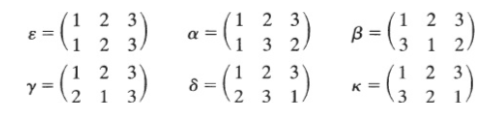
\includegraphics[width = \textwidth]{permSetExample}$$ 
Then $\beta$ is the function such that $\beta(1) = 3$, $\beta(2) = 1$ and $\beta(3) = 2$. The operation on elements of $S_3$ is composition. To find $\alpha \circ \beta$, note that $$\begin{aligned} [\alpha \circ \beta](1) &= \alpha(\beta(1)) = \alpha(3) = 2 \\ [\alpha \circ \beta](2) &= \alpha(\beta(2)) = \alpha(1) = 2 \\ [\alpha \circ \beta](3) &= \alpha(\beta(3)) = \alpha(2) = 3 \end{aligned} $$ 
Thus $$\alpha \circ \beta = \begin{pmatrix} 1 & 2 & 3 \\ 2 & 1 & 3 \end{pmatrix} = \gamma $$ 
Note that in $\alpha \circ \beta$, $\beta$ is applied first and $\alpha$ next. \\ Here is the table of the group $S_3$ 
$$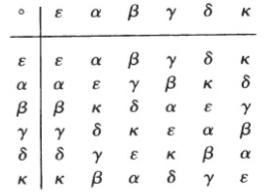
\includegraphics{groupS3}$$ \end{example} 
 
\begin{definition} The inverse of any permutation of $A$ is a permutation of $A$. Furthermore, if $f$ is any permutation of $A$ and $\inverse{f}$ is its inverse, then $$\inverse{f} \circ f = \varepsilon \text{ and } f \circ \inverse{f} = \varepsilon $$ \end{definition} 

\begin{definition} For any set $A$, the group of all the permutations of $A$ is called the symmetric group on $A$, represented by $S_A$ \end{definition} 

\begin{definition} For any positive integer $n$, the symmetric group on the set $\set{1, 2, 3, \dots, n}$ is called the symmetric group on $n$ elements, denoted by $S_n$ \end{definition} 

\begin{example} Group of Symmetries of the Square: Think of a symmetry of the square as any way of moving a square to make it coincide with its former position. Every time we do this, vertices will coincide with vertices, so a symmetry is completely described by its effect on the vertices. \\ Number the vertices as follows: $$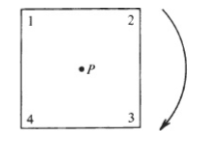
\includegraphics{squaresym}$$ 
The most obvious symmetries are obtained by rotating the square clockwise around its center $P$, through angles of $90^{\circ}$, $180^{\circ}$ and $270^{\circ}$ respectively. Each symmetry is indicated as a permutation of the vertices, thus a clockwise rotation of $90^{\circ}$ yields the symmetry $$R_1 = \begin{pmatrix} 1 & 2 & 3 & 4 \\ 2 & 3 & 4 & 1 \end{pmatrix} $$ 
for this rotation carries vertex 1 to 2, 2 to 3, 3 to 4 and 4 to 1. Rotations of $180^{\circ}$ and $270^{\circ}$ yield the following symmetries respectively $$ R_2 = \begin{pmatrix} 1 & 2 & 3 & 4 \\ 3 & 4 & 1 & 2 \end{pmatrix} ~~ R_3 = \begin{pmatrix} 1 & 2 & 3 & 4 \\ 4 & 1 & 2 & 3 \end{pmatrix} $$ The remaining symmetries are flips of the square about its axes $A,~B,~C$ and $D$ as follows 
$$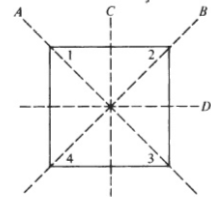
\includegraphics{squaresymtwo}$$ When the square is flipped about the axis $A$, vertices 1 and 3 stay put but 2 and 4 change places to get the following symmetry $$R_4 = \begin{pmatrix} 1 & 2 & 3 & 4 \\ 1 & 4 & 3 & 2 \end{pmatrix} $$ In the same way, the other flips are $$ R_5 = \begin{pmatrix} 1 & 2 & 3 & 4 \\ 3 & 2 & 1 & 4 \end{pmatrix} ~~ R_6 = \begin{pmatrix} 1 & 2 & 3 & 4 \\ 2 & 1 & 4 & 3 \end{pmatrix} $$ and $$ R_7 = \begin{pmatrix} 1 & 2 & 3 & 4 \\ 4 & 3 & 2 & 1 \end{pmatrix} $$ The last symmetry is the identity $$R_0 = \begin{pmatrix} 1 & 2 & 3 & 4 \\ 1 & 2 & 3 & 4 \end{pmatrix}$$ which leaves the square as it is. \\sim\\
The operation on symmetries is composite; $R_i \circ R_j$ is the result of first performing $R_j$ and then $R_i$. For example, $R_1 \circ R_4$ is the result of first flipping the square about its axis $A$ and then rotating it clockwise $90^{\circ}$ $$ \begin{aligned} R_1 \circ R_4 &= \begin{pmatrix} 1 & 2 & 3 & 4 \\ 2 & 3 & 4 & 1 \end{pmatrix} \circ \begin{pmatrix} 1 & 2 & 3 & 4 \\ 1 & 4 & 3 & 2 \end{pmatrix} \\ &= \begin{pmatrix} 1 & 2 & 3 & 4 \\ 2 & 1 & 4 & 3 \end{pmatrix} = R_6 \end{aligned} $$ Thus the net effect is the same as if the square had been flipped about its axis $C$. \\sim\\ The eight symmetries of the square form a group under the operation $\circ$ of composition, called the group of symmetries of the square. \end{example} 

\begin{definition} For every positive integer $n \geq 3$, the regular polygon with $n$ sides has a group of symmetries, symbolized by $D_n$. The groups are called the dihedral groups. \end{definition} 


\section{Permutations of a Finite Set}

\begin{definition} If $n$ is a positive integer, consider a set of $n$ elements, $\set{1, 2, \dots, n}$. The group of all the permutations of this set is called the symmetric group on $n$ elements and is denoted by $S_n$. \end{definition} 

\begin{example} $f$ is the permutation as follows $$ f = \begin{pmatrix} 1 & 2 & 3 & 4 & 5 & 6 & 7 & 8 & 9 \\ 3 & 1 & 6 & 9 & 8 & 2 & 4 & 5 & 7 \end{pmatrix} $$ 
$f$ moves the elements in its domain as follows: $$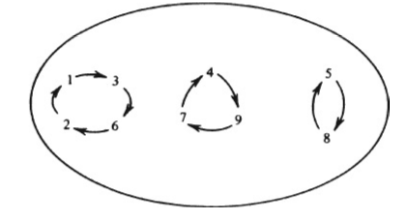
\includegraphics{permcycle}$$ Note how $f$ decomposes its domain into three separate subsets, so that, in each subset, the elements are permuted cyclically so as to form a closed chain. \end{example} 

\begin{definition} Let $a_1, a_2, \dots, a_s$ be distinct elements of the set $\set{1, 2, \dots, n}$. By the cycle $(a_1a_2\dots a_s)$ we mean the permutation $$a_1 \to a_2 \to a_3 \to \dots \to a_{s_1} \to a_s \to a_1$$ and so forth of $\set{1, 2, \dots, n}$ which carries $a_1$ to $a_2$, $a_2$ to $a_3$, ,,,, $a_{s - 1}$ to $a_s$ and $a_s$ to $a_1$, which leaving all the remaining elements of $\set{1, 2, \dots, n}$ fixed. \end{definition}

\begin{example} In $S_6$, the cycle (1246) is the permutation $$\begin{pmatrix} 1 & 2 & 3 & 4 & 5 & 6 \\ 4 & 6 & 3 & 2 & 5 & 1 \end{pmatrix} $$ In $S_5$, the cycle (254) is the permutation $$\begin{pmatrix} 1 & 2 & 3 & 4 & 5 \\ 1 & 5 & 3 & 2 & 4 \end{pmatrix} $$ \end{example} 

\begin{definition} The composite of cycles is generally called the product and it is customary to omit the symbol $\circ$ \end{definition} 

\begin{example} In $S_5$, $$\begin{aligned} (254)(124) &= \begin{pmatrix} 1 & 2 & 3 & 4 & 5 \\ 1 & 4 & 3 & 5 & 2 \end{pmatrix} \circ \begin{pmatrix} 1 & 2 & 3 & 4 & 5 \\ 2 & 4 & 3 & 1 & 5 \end{pmatrix} \\ &= \begin{pmatrix} 1 & 2 & 3 & 4 & 5 \\ 4 & 5 & 3 & 1 & 2 \end{pmatrix} \end{aligned} $$ It is very easy to compute the product of two cycles by reasoning in the following manner.$$ (\underbrace{2 ~ 4 ~ 5}_{\alpha})(\underbrace{1 ~ 2 ~ 4}_{\beta}) $$ 
Remember that the permutation on the right is applied first and the permutation on the left is applied next. Now, \\ $\beta$ carries 1 to 2, and $\alpha$ carries 2 to 4; hence $\alpha\beta$ carries 1 to 4 \\ $\beta$ carries 2 to 4, and $\alpha$ carries 4 to 5; hence $\alpha\beta$ carries 2 to 5 \\ $\beta$ carries 3 fixed and so does $\alpha$; hence $\alpha\beta$ leaves 3 fixed \\ $\beta$ carries 4 to 1 and $\alpha$ leaves 1 fixed; so $\alpha\beta$ carries 4 to 1 \\ $\beta$ leaves 5 fixed and $\alpha$ carries 5 to 2; hence $\alpha\beta$ carries 5 to 2 \end{example} 

\begin{definition} If $(a_1a_2\dots a_s)$ is a cycle, the integer $s$ is called its length; thus $(a_1a_2\dots a_s)$ is a cycle of length $s$ \end{definition} 

\begin{definition} If two cycles have no elements in common they are said to be disjoint \end{definition} 

Note: Disjoint cycles comment; that is, if $(a_1\dots a_r)$ and $(b_1\dots b_s)$ are disjoint, then $$(\underbrace{a_1\dots a_r}_{\alpha})(\underbrace{b_1\dots b_s}_{\beta}) = (\underbrace{b_1\dots b_s}_{\beta})(\underbrace{a_1\dots a_r}_{\alpha}) $$ 

\begin{theorem} Every permutation is either the identity, a single cycle, or a product of disjoint cycles \end{theorem} 

\begin{example} Consider the permutation $$f = \begin{pmatrix} 1 & 2 & 3 & 4 & 5 & 6 \\ 3 & 4 & 5 & 2 & 1 & 6 \end{pmatrix} $$ and let us write $f$ as a product of disjoint cycles. We begin with 1 and note that $$ 1 \overset{f}{\rightarrow} 3 \overset{f}{\rightarrow} 5 \overset{f}{\rightarrow} 1 $$
This is a complete cycle, which is (135). Next, take the first number which hasn't yet been used, namely, 2. We see that $$2 \overset{f}{\rightarrow} 4 \overset{f}{\rightarrow} 2 $$ This is a complete cycle, (24). The only remaining number is 6, which is fixed. Thus $$ f = (135)(24)$$ \end{example}  

Note: The product of cycles is unique, except for the order of the factors. 

\begin{definition} A cycle of length 2 is called a transposition. In other words, a transposition is a cycle $(a_i, a_j)$ which interchanges the two numbers $a_i$ and $a_j$. Every cycle can be expressed as a product of one or more transpositions. in fact, $$ (a_1a_2 \dots a_r) = (a_ra_{r - 1})(a_ra_{r - 2}) \dots (a_ra_3)(a_ra_2)(a_ra_1)$$  \end{definition} 

\begin{example} Note the following $$ \begin{aligned} (12345) &= (54)(53)(52)(41) \\ &= (15)(14)(13)(12) \\ &= (54)(52)(51)(14)(32)(41) \end{aligned} $$ This shows that every permutation, after it has been decomposed into disjoint cycles, may be broken down further and expressed as a product of transpositions. However, the expression as a product of transpositions is not unique and even the number of transpositions involved is not unique. \end{example} 

\begin{definition} A permutation is called even if it is a product of an even number of transpositions and odd if it is a product of odd number of transpositions \end{definition} 

\begin{theorem} No matter how $\varepsilon$ is written as a product of transpositions, the number of transpositions is even \end{theorem} 

\begin{theorem} If $\pi \in S_n$, then $\pi$ cannot be both an odd permutation and an even permutation \end{theorem} 

\begin{definition} The set of all the even permutations in $S_n$ is a subgroup of $S_n$. It is denoted by $A_n$ and is called the alternating group on the set $\set{1, 2, \dots, n}$ \end{definition} 

\section{Isomorphism}

\begin{definition} If $G_1$ and $G_2$ are any groups, an isomorphism from $G_1$ to $G_2$ is a one-to-one correspondence $f$ from $G_1$ to $G_2$ with the following property: For every pair of elements $a$ and $b$ in $G_1$, $$\text{If } f(x) = a' \text{ and } f(b) = b' \text{ then } f(ab) = a'b' $$ 
In other words, let $G_1$ and $G_2$ be groups. A bijective function $f: G_1 \to G_2$ with the property that for any two elements $a$ and $b$ in $G_1$, $$f(ab) = f(a)f(b)$$ is called an isomorphism from $G_1$ to $G_2$. \end{definition} 

\begin{definition} If there exists an isomorphism from $G_1$ to $G_2$, then $G_1$ is isomorphic to $G_2$ and can be written as $$G_1 \cong G_2$$ \end{definition} 

To Recognize if Two Groups are Isomorphic: \begin{enumerate} 
\item Make an educated guess and come up with a function $f: G_1 \mathcal{F} G_2$ which looks as though it might be an isomorphism 
\item Check that $f$ is injective and surjective
\item Check that $f$ satisfies the identity $$f(ab) = f(a)f(b)$$ \end{enumerate} 

\begin{example} $\reals$ under addition \end{example} 

To Recognize if Two Groups are not Isomorphic: \begin{enumerate} 
\item Perhaps $G_1$ is commutative and $G_2$ is not 
\item Perhaps $G_1$ has an element which is its own inverse and $G_2$ does not 
\item Perhaps $G_1$ is generated by two elements whereas $G_2$ is not generated by any choice of two of its elements 
\item Perhaps every element of $G_1$ is the square of an element of $G_1$ whereas $G_2$ does not have this property \end{enumerate} 
Note: This list is not exhaustive. Be on the lookout for properties which do not depend merely on the names assigned to individual elements. 

\begin{definition} If $G_1$ and $G_2$ cannot be put in one-to-one correspondence (say $G_1$ has more elements than $G_2$), clearly they cannot be isomorphic. \end{definition} 

\begin{theorem} Cayley's Theorem: Every group is isomorphic to a group of permutations. \end{theorem} 

\section{Order of Group Elements}

\begin{definition} Let $G$ be an arbitrary group, with its operation denoted multiplicatively. Exponential notation is a convenient shorthand: for any positive integer $n$, let $$a^n = \underbrace{a \cdot a \cdot \dots \cdot a}_{n \text{ times }}$$ $$a^{-n} = \underbrace{\inverse{a} \inverse{a} \dots \inverse{a}}_{n \text{ times }} $$ and $$a^0 = e$$ \end{definition} 

\begin{theorem} Laws of Exponents: If $G$ is a group and $a \in G$, the following identities hold for all integers $m$ and $n$: 
\begin{itemize} 
\item $a^ma^n = a^{m + n}$
\item $(a^m)^n = a^{mn}$
\item $a^{-n} = (a^{-1})^n = \pinverse{a^n}$ \end{itemize} \end{theorem} 

\begin{theorem} Division Algorithm: If $m$ and $n$ are integers and $n$ is positive, there exist unique integers $q$ and $r$ such that $$m = nq + r \text{ and } 0 \geq r < n $$ $q$ is called the quotient and $r$ is the remainder in the division of $m$ by $nx$. \end{theorem} 

\begin{definition} Let $G$ be a group and $a$ an element of $G$. If there exists a nonzero integer $m$ such that $a^m = e$, then there exists a positive integer $n$ such that $a^n = e$. \end{definition} 

\begin{definition} If there exists a nonzero integer $m$ such that $a^m = e$, then the order of the element $a$ is defined to be the least positive integer $n$ such that $a^n = e$. If there does not exist any nonzero integer $m$ such that $a^m = e$, then $a$ has order infinity. \end{definition} 

Note: In $\integers$, every nonzero number has infinite order. 

\begin{theorem} Let $G$ be an arbitrary group and $a$ is any element of $G$. If the order of $a$ is $n$, there are exactly $n$ different powers of $a$, namely $$a^0,a, a^2, a^3, \dots, a^{n-1}$$ \end{theorem} 

\begin{theorem} Let $G$ be an arbitrary group and $a$ is any element of $G$. Suppose an element $a$ in the group $G$ has order $n$. Then $a^t = e$ if and only if $t$ is a multiple of $n$. \end{theorem} 

\section{Cyclic Groups}

\begin{definition} If $G$ is a group and $a \in G$, it may happen that every element of $G$ is a power of $a$. $$G = \set{a^n: n \in \integers}$$ In that case, $G$ is called a cyclic group and $a$ is called its generator. $$G = <a>$$ \end{definition} 

\begin{definition} If $G = <a>$ is the cyclic group generated by $a$ and $a$ has order $n$, then $G$ is a cyclic group of order $n$. If the generator of $G$ has order infinity, then $G$ is cyclic group of order infinity. \end{definition} 

\begin{theorem} Isomorphism of Cyclic Groups \begin{enumerate} 
\item For every positive integer $n$, every cyclic group of order $n$ is isomorphic to $\integers_n$. thus, any two cyclic groups of order $n$ are isomorphic to each other. 
\item Every cyclic group of order infinity is isomorphic to $\integers$ and therefore any two cyclic groups of order infinity are isomorphic to each other. \end{enumerate} \end{theorem} 

If $G$ is any group and $a \in G$, it is easy to see that \begin{itemize} 
\item The product of any two powers of $a$ is a power of $a$: $a^ma^n = a^{m + n}$
\item The inverse of any power of $a$ is a power of $a$ because $\pinverse{a^n} = a^{-n}$ 
\item The set of all the powers of $a$ is a subgroup of $G$ \end{itemize} 
This subgroup is called the cyclic subgroup of $G$ generated by $a$. 

\begin{theorem} Every subgroup of a cyclic group is cyclic. \end{theorem} 

\begin{definition} Let $a$ be an element of order $n$ in a group $G$. There are exactly $n$ different powers of $a$, hence $<a>$ has $n$ elements. Thus, if ord($a) = n$, then $|<a>| = n$. That is, the order of a cyclic group is the same as the order of its generator. \end{definition} 

\section{Partitions and Equivalence Relations} 

\begin{definition} By a partition of a set $A$, we mean a family $\set{A_i: i \in I}$ of nonempty subsets of $A$ such that: \begin{itemize} 
\item If any two classes, say $A_i$ and $A_j$, have a common element $x$ (that is, are not disjoint), then $A_i = A_j$ and 
\item Every element $x$ of $A$ lies in one of the classes \end{itemize}  \end{definition} 

By an equivalence relation on a set $A$, we mean a relation $\sim$ which is: \begin{itemize} 
\item Reflexive: that is, $x \sim x$ for every $x$ in $A$ 
\item Symmetric: that is, if $x \sim y$, then $y \sim x$
\item Transitive: that is, if $x \sim y$ and $y\sim z$ then $x \sim z$ \end{itemize} 

Note: Two elements are ``equivalent'' if they are members of the same class. 

\begin{definition} Let $\sim$ be an equivalence relation on $A$ and $x$ an element of $A$. The set of all the elements equivalent to $x$ is called the equivalence class of $x$ and is denoted by $[x]$. In symbols, 
$$[x] = \set{y \in A: y \sim x}$$ \end{definition} 

Property: If $x \sim y$, then $[x] = [y]$. In other words, if two elements are equivalent, they have the same equivalence class. 

\begin{theorem} If $\sim$ is an equivalence relation on $A$, the family of all the equivalence classes, that is, $\set{[x]: x \in A}$, is a partition on $A$. \end{theorem} 

When $\sim$ is an equivalence relation on $A$ and $A$ is partitioned into its equivalence classes, this partition is called the partition determined by the equivalence relation $\sim$. 


\section{Counting Cosets}

\begin{definition} Let $G$ be a group and $H$ a subgroup of $G$. For any element $a$ in $G$, the symbol $$aH$$ denotes the set of all products $ah$, as $a$ remains fixed and $h$ ranges over $H$. $aH$ is called a left coset of $H$ in $H$. \\ In similar fashion $$Ha$$ denotes the set of all products $ha$ as $a$ remains fixed and $h$ ranges over $H$. $Ha$ is called a right coset of $H$ in $G$. \end{definition} 

Note: It will not make a difference which coset you use as long as you are consistent. \\
Fact: Every coset in group $G$ is a subset of $G$. To prove that two cosets $Ha$ and $Hb$ are equal, show that they are equal sets; which means, show that every element $x \in Ha$ is in $Hb$ and every element $y \in Hb$ is in $Ha$. \\~\\
Fact: If $a \in Hb$, then $Ha = Hb$. 

\begin{theorem} The family of all the cosets $Ha$, as $a$ ranges over $G$, is a partition of $G$. \end{theorem} 

\begin{theorem} If $Ha$ is any coset of $H$, there is a one-to-one correspondence from $H$ to $Ha$. \\ A consequence of this is that all cosets of $H$ have the same number of elements. \end{theorem} 

Note: The number of elements in $G$ is equal to the number of elements in $H$, multiplied by the number of distinct cosets of $H$. 

\begin{theorem} Lagrange's Theorem: Let $G$ be a finite group and $H$ any subgroup of $G$. The order of $G$ is a multiple of the order of $H$. \end{theorem} 

\begin{theorem} If $G$ is a group with a prime number $p$ of elements, then $G$ is a cyclic group. Furthermore, any element $a \neq e$ in $G$ is a generator of $G$. \end{theorem} 

\begin{theorem} The order of any element of a finite group divides the order of the group. \end{theorem} 

\begin{definition} If $G$ is a group and $H$ is a subgroup of $G$, the index of $H$ in $G$ is the number of cosets of $H$ in $G$, denoted by  $(G:H)$. Since the number of elements in $G$ is equal to the number of elements in $H$, multiplied by the number of cosets of $H$ in $G$, $$(G:H) = \frac{\text{order of }G}{\text{order of }H}$$ \end{definition} 

\section{Homomorphisms}

\begin{definition} If $G$ and $H$ are groups, a homomorphism from $G$ to $H$ is a function $f: G \to H$ such that for any two elements $a$ and $b$ in $G$, $$f(ab) = f(a)f(b)$$ If there exists a homomorphism from $G$ onto $H$, then $H$ is a homomorphic image of $G$. \end{definition} 

\begin{theorem} Let $G$ and $H$ be groups and $f: G \to H$ a homomorphism. Then \begin{enumerate} 
\item $f(e) = e$ 
\item $f(\inverse{a}) = [f(a)]^{-1}$ for every element $a \in G$ \end{enumerate} \end{theorem} 

\begin{definition} Let $H$ be a subgroup of a group $G$. $H$ is called a normal subgroup of $G$ if it is closed with respect to conjugates, that is, if $$ \text{for any } a \in H \text{ and } x \in G \text{ then } xa\inverse{x} \in H $$ \end{definition} 

\begin{definition} Let $f: G \to H$ be a homomorphism. The kernel of $f$ is the set $K$ of all the elements of $G$ which are carried by $f$ onto the neutral element of $H$. That is, $$ K = \set{x \in G: f(x) = e}$$ \end{definition} 

\begin{theorem} Let $f: G \to H$ be a homomorphism. \begin{enumerate} 
\item The kernel of $f$ is a normal subgroup of $G$
\item The range of $f$ is a subgroup of $H$ \end{enumerate} \end{theorem} 

Note: If $f$ is a homomorphism, the kernel of $f$ and the range of $f$ are represented as follows $$ \text{ker}(f) \text{  and  } \text{ran}(f) $$ 

\section{Quotient Groups}

\begin{theorem} If $H$ is a normal subgroup of $G$, then $aH = Ha$ for every $a \in G$. \end{theorem} 
In other words, there is no distinction between left and right cosets for a normal subgroup. 

\begin{definition} Coset Multiplication: Let $G$ be a group and let $H$ be a subgroup of $G$. The coset of $a$, multiplied by the coset of $b$, is defined to be the coset of $ab$ $$Ha \cdot Hb = H(ab)$$ \end{definition} 

\begin{theorem} Let $H$ be a normal subgroup of $G$. If $Ha = He$ and $Hb = Hd$, then $H(ab) = H(cd)$. \end{theorem} 

\begin{definition} Let $G$ be a group and let $H$ be a normal subgroup of $G$. The set consisting of all the cosets of $H$ is denoted by the symbol $G/H$. Thus if $Ha$, $Hb$, $He$, $\dots$, are cosets of $H$ then $$G/H = \set{Ha, Hb, Hc, \dots}$$ \end{definition} 

\begin{theorem} $G/H$ with coset multiplication is a group. \end{theorem} 

\begin{definition} The group $G/H$ is called the factor group, or quotient group of $G$ by $H$. \end{definition} 

\begin{theorem} $G/H$ is a homomorphic image of $G$. \end{theorem} 

\begin{theorem} Let $G$ be a group and $H$ a subgroup of $G$. Then  \begin{enumerate} 
\item $Ha = Hb$ iff $a\inverse{b} \in H$ 
\item $Ha = H$ iff $a \in H$ \end{enumerate} \end{theorem} 

\begin{definition} Let $G$ be an arbitrary group; by a commutator of $G$, we mean any element of the form $ab\inverse{a}\inverse{b}$ where $a$ and $b$ are in $G$ $$ ab\inverse{a}\inverse{b} = e \text{ iff } ab = ba $$ In other words, $ab\inverse{a}\inverse{b}$ reduces to the neutral element whenever $a$ and $b$ commute. \end{definition} 

Note: When we factor out the commutators of $G$, we get a quotient group which has no commutators and is therefore abelian. 

\begin{definition} To say that $G/H$ is abelian is to say that any two elements $Hx$ and $Hy$ in $G/H$, $HxHy = HyHx$; that is, $Hxy = Hyx$. But $$Hxy = Hyx \text{ iff } xy\pinverse{yx} \in H $$ Now $xy\pinverse{yx}$ is the commutator $xy\inverse{x}\inverse{y}$; so if all commutators are in $H$ then $G/H$ is abelian. \end{definition} 

\section{The Fundamental Homomorphism Theorem}

Let $G$ be any group. Every quotient group of $G$ is a homomorphic image of $G$. It is also true that ever homomorphic image of $G$ is isomorphic to a quotient group of $G$. It follows that, for any groups $G$ and $H$, $H$ is a homomorphic image of $G$ iff $H$ is (or is isomorphic to) a quotient group of $G$. 

\begin{theorem} Let $f: G \to H$ be a homomorphism with kernel $K$. Then $$f(a) = f(b) \text{ iff } Ka = Kb$$ In other words, any two elements $a$ and $b$ in $G$ have the same image under $f$ iff they are in the same coset of $K$. \end{theorem} 

This says that if $f$ is a homomorphic from $G$ to $H$ with kernel $K$, then all the elements in any fixed coset of $K$ have the same image, and conversely, elements which have the same image are in the same coset of $K$. 

\begin{theorem} Let $f: G \to H$ be a homomorphism of $G$ onto $H$. If $K$ is the kernel of $f$, then $$H \cong G/K $$ \end{theorem} 

The above theorem is often called the Fundamental Homomorphism Theorem. It asserts that every homomorphic image of $G$ is isomorphic to a quotient group of $G$. Which specific quotient group of $G$? If $f$ is a homomorphism from $G$ onto $H$, then $H$ is isomorphic to the quotient group of $G$ by the kernel of $f$. \\~\\
Note: The fact that $f$ is a homomorphism from $G$ onto $H$ may be symbolized by writing $$f: G \twoheadrightarrow H$$ Furthermore, the fact that $K$ is the kernel of this homomorphism may be indicated by writing $$f: G \twoheadrightarrow_K H$$ Thus, the fundamental homomorphism theorem says that 
$$ \text{If } f: G \twoheadrightarrow_K H \text{ then } H \cong G/H $$ 

\section{Rings: Definitions and Elementary Properties}

\begin{definition} By a ring, we mean a set $A$ with operations called addition and multiplication which satisfy the following axioms: \begin{enumerate} 
\item $A$ with addition alone is an abelian group
\item Multiplication is associative
\item Multiplication is distributive over addition. That is, for all $a$, $b$, and $c$ in $A$, $$a(b+c) = ab + ac$$ and $$(b+c)a = ba + ca$$ \end{enumerate} \end{definition} 
Note: Since $A$ with addition alone is an abelian group, there is in $A$ a neutral element for addition called the zero element and is written $0$. Also, every element has an additive inverse called its negative; the negative of $a$ is denoted by $-a$. 

\begin{example} The set $\integers$ of the integers, with conventional addition and multiplication, is a ring called the ring of the integers and is denoted $\integers$. Similarly, $\rationals$ is the ring of rational numbers, $\reals$ is the ring of the real numbers and $\complex$ is the ring of the complex numbers, each under conventional addition and multiplication. \end{example} 

\begin{example} $\mathcal{F}(\reals)$ represents the set of all the functions from $\reals$ to $\reals$ and with the operation of addition and multiplication of functions, it is a ring, called the ring of real functions. \end{example}

\begin{definition} The rings $\integers$, $\rationals$, $\reals$, $\complex$ and $\mathcal{F}(\reals)$ are all infinite rings, that is, rings with infinitely many elements. \\ There are also finite rings: rings with a finite number of elements. Examples of these are $\integers_n$. \end{definition} 

Note: Let $A$ be any ring. Since $A$ with addition alone is an abelian group, the following is true for ring $A$ $$ \begin{aligned} a + b = a + c &\text{ implies } b = c \\ a + b = 0 &\text{ implies } a = -b \text{ and } b = -a \\ -(a + b) --a + -b &\text{ and } -(-a) = a \end{aligned} $$ These statements are true in every ring, 

\begin{theorem} Let $a$ and $b$ be any elements of a ring $A$. \begin{enumerate} 
\item $a0 = 0$ and $0a = 0$ 
\item $a(-b) = -(ab)$ and $(-a)b = -(ab)$ 
\item $(-a)(-b) = ab$ \end{enumerate} \end{theorem} 

\begin{definition} By definition, addition is commutative in every ring but multiplication is not. When multiplication also is commutative in a ring, that ring is called a commutative ring. \end{definition} 

\begin{definition} If there is in ring $A$ a neutral element for multiplication, it is called the unity of $A$ and is denoted by the symbol $1$. Thus $a \cdot 1 = a$ and $1 \cdot a = a$ for every $a$ in $A$. If $A$ has a unity, $A$ is a ring with unity. \end{definition} 

\begin{example} The rings $\integers$, $\rationals$, $\reals$, $\complex$ and $\mathcal{F}$ are all examples of commutative rings with unity. \end{example} 

\begin{definition} A ring whole only element is $0$ is called a trivial ring; a ring with more than one element is nontrivial. In a nontrivial ring with unity, necessarily $1 \neq 0$. This is true because if $1 = 0$ and $x$ is any element of the ring, then $$x = x1 = x0 = 0$$ In other words, if $1 = 0$ then every element of the ring is equal to $0$; hence $0$ is the only element of the ring. \end{definition} 

\begin{definition} If $A$ is a ring with unity, they may be elements in $A$ which have a multiplicative inverse. Such elements are said to be invertible. Thus, an element $a$ is invertible in a ring if there is some $x$ in the ring such that $$ax = xa = 1$$ \end{definition} 

Note: Zero is never an invertible element of a ring except if the ring is trivial. 

\begin{definition} If $A$ is a commutative ring with unity in which every nonzero element is invertible, $A$ is called a field. \end{definition} 

\begin{example} $\rationals$, $\reals$ and $\complex$ are fields. \end{example} 

\begin{definition} In any ring, a nonzero element $a$ is called a divisor of zero if there is a nonzero element $b$ in the ring such that the product $ab$ or $ba$ is equal to zero. \end{definition} 

Note: $\integers$, $\rationals$, $\reals$ and $\complex$ do not have any divisors of zero. 

\begin{definition} A ring is said to have the cancellation property if $$ab = ac \text{ or } ba = ca \text{ implies } b = c $$ for any elements $a$, $b$, and $c$ in the ring if $a \neq 0$. \end{definition} 

\begin{theorem} A ring has the cancellation property if and only if it has no divisors of zero. \end{theorem} 

\begin{definition} An integral domain to defined to be a commutative ring with unity having the cancellation property. It may also be defined as a commutative ring with ring having no divisors of zero. \end{definition} 

Note: If is easy to see that every field is an integral domain. The converse is not true though. 

\begin{example} $\integers$ is an integral domain but not a field. \end{example} 

\section{Ideals and Homomorphisms}

\begin{definition} If a nonempty subset $B \subseteq A$ is closed with respect to addition, multiplication and negatives, then $B$ with the operations of $A$ is a ring. \end{definition} 

\begin{definition} $B$ is a subring of $A$ if and only if $B$ is closed with respect to subtraction and multiplication. \end{definition} 

\begin{definition} Let $A$ be a ring and $B$ a nonempty subset of $A$. $B$ is called an ideal of $A$ if $B$ is closed with respect to addition and negatives and $B$ absorbs products in $A$
$$ \forall b \in B \text{ and } x \in A, xb \text{ and } bx \text{ are in } B $$ 
\end{definition} 

\begin{example} In a commutative ring with unity, the simplest example of an ideal is the set of all the multiplies of a fixed element $a$ by all the elements in the ring. In other words, the set of all the products $xa$ as $a$ remains fixed and $x$ ranges over all the elements of the ring. this set is an ideal because $$xa + ya = (x+y)a$$ $$-(xa) = (-x)a$$ and $$y(xa) = (yx)a$$ This ideal is called the principal ideal generated by $a$ and is denoted by $\langle a \rangle$. \end{example}

\begin{definition} If $B$ is a nonempty subset of $A$ then $B$ is an ideal of $A$ if and only if $B$ is closed with respect to subtraction and $B$ absorbs products in $A$. \end{definition} 

\begin{definition} A homomorphism from a ring $A$ to a ring $B$ is a function $f: A \to B$ satisfying the identities $$ \begin{aligned} f(x_1 + x_2) &= f(x_1) + f(x_2) \\ f(x_1x_2) &= f(x_1)f(x_2) \end{aligned} $$ \end{definition} 

Note: If there is a homomorphism from $A$ onto $B$, we call $B$ a homomorphic image of $A$. If $f$ is a homomorphism from a ring $A$ to a ring $B$, not necessarily onto, the range is a subring of $B$. Thus, the range of a ring homomorphism is always a ring. 

\begin{definition} If $f$ is a homomorphism from a ring $A$ to a ring $B$, the kernel of $f$ is the set of all the elements of $A$ which are carried by $f$ onto the zero element of $B$. In symbols, the kernel of $f$ is the set $$ K = \{ x \in A : f(x) = 0\} $$ Note: The kernel of $f$ is an ideal of $A$. \end{definition} 

\begin{definition} If $A$ and $B$ are rings, an isomorphism from $A$ to $B$ is a homomorphism which is a one-to-one correspondence from $A$ to $B$. In other words, it is an injective and surjective homomorphism. If there is an isomorphism from $A$ to $B$, then $A$ is isomorphic to $B$ $$ A \cong B$$ \end{definition} 

\section{Quotient Rings}

\begin{definition} Let $A$ be a ring and $J$ an ideal of $A$. For any elements $a \in A$, the symbol $J + a$ denotes the set of all sums $j+a$ as $a$ remains fixed and $j$ ranges over $J$. That is, $$ J + a = \{j + a: j \in J\}$$ $J+a$ is called a coset of $J$ in $A$. \end{definition} 

If we provisionally ignore multiplication, $A$ with addition alone is an abelian group and $J$ is a subgroup of $A$. Thus, the cosets are precisely the cosets of the subgroup $J$ in the group $A$, with the notation being additive. In additive notation: $$ \begin{aligned} a \in J + b &\iff J + a = J + b \\ J + a = J + b &\iff a - b \in J \\ J + a = J &\iff a \in J \end{aligned} $$ 
By the reasoning which lead up to Lagrange's Theorem, the family of all the cosets $J + a$ as $a$ ranges over $A$, is a partition of $A$. \\
There is a way of adding and multiplying cosets which works as follows: $$ \begin{aligned} (J + a) + (J + b) &= J + (a + b) \\ (J + a)(J + b) &= J + ab \end{aligned} $$ In other words, the sum of the coset of $a$ and the coset of $b$ is the coset of $a+b$; the product of the coset of $a$ and the coset of $b$ is the coset of $ab$. 

\begin{theorem} Let $J$ be an ideal of $A$. If $J + a = J+c$ and $J+b = J+d$, then \begin{enumerate} 
\item $J + (a + b) = J + (c + d) $ 
\item $J + ab = J + cd $ \end{enumerate} \end{theorem} 

\begin{definition} The set which consists of all the cosets of $J$ in $A$ is $$ A/J = \{J+a, J+b, J+c, \dots\}$$ \end{definition} 

\begin{theorem} $A / J$ with coset addition and multiplication is called the quotient ring of $A$ by $J$. \end{theorem} 

\begin{theorem} $A/J$ is a homomorphic image of $A$. \end{theorem} 

\begin{definition} The natural homomorphism from $A$ onto $A/J$ is the function $f$ which carries every element to its own coset, that is, the function $f$ given by $$f(x) =  J + x $$ \end{definition} 

\begin{theorem} Fundamental Homomorphism Theorem for Rings: Let $f: A \to B$ be a homomorphism from a ring $A$ onto a ring $B$ and let $K$ be the kernel of $f$. Then $ B \cong A/K$. \end{theorem} 

Therefore, every quotient ring of $A$ is a homomorphic image of $A$ and conversely, every homomorphic image of $A$ is isomorphic to a quotient ring of $A$. Thus, quotients and homomorphic images of a ring are the same. 
\\~\\
 Let $A$ be a ring and let $J$ be an ideal of $A$ which contains all the differences $ab - ba$ as $a$ and $b$ ranges over $A$. Then $A/J$ is commutative. In other words, for any two cosets $J+a$ and $J+b$, $$(J+a)(J+b) = (J+b)(J+a) \text{ that is } J + ab = J + ba $$ 
This is true if and only if $ab - ba \in J$ Thus, if every difference $ab - ba \in J$, then any two cosets commute. 

\begin{definition} An ideal $J$ of a commutative ring is said to be a prime ideal if for any two elements $a$ and $b$ in the ring, if $ab \in J$ then $a \in J$ or $b \in J$. Note: Whenever $J$ is a prime ideal of a commutative ring with unity $A$, the quotient ring $A/J$ is an integral domain. \end{definition} 

\begin{definition} An ideal of a ring is called proper if it is not equal to the whole ring. \end{definition} 

\begin{definition} A proper ideal of a ring $A$ is called a maximal ideal if there exists no proper ideal $K$ of $A$ such that $J \subseteq K$ with $J \neq K$. \end{definition} 

Note: If $A$ is a commutative ring with unity, then $J$ is a maximal ideal of $A$ if and only if $A/J$ is a field. 

%\section{Integral Domains}

%\section{The Integers}

\section{Factoring into Primes}

\begin{theorem} Every ideal of $\integers$ is principal. \end{theorem} 

\begin{definition} If $r$ and $s$ are integers, then $s$ is a multiple of $r$ if there is an integer $k$ such that $$s = rk$$ If this is the case, then $r$ is a factor of $s$, or $r$ divides $s$, denoted by $$r|s$$ \end{definition} 

\begin{theorem} The only invertible elements of $\integers$ are $1$ and $-1$. \end{theorem} 

\begin{definition} A pair of integers $r$ and $s$ are called associates if they divide each other, that is, if $r|s$ and $s|r$. If $r$ and $s$ are associates, this means there are integers $k$ and $l$ such that $r = ks$ and $s = lr$. Thus $r = ks = klr$, hence $kl = 1$. By the above theorem, $k$ and $l$ are $\pm 1$ and therefore $r = \pm s$. Thus, if $r$ and $s$ are associates in $\integers$, then $r = \pm s$. \end{definition} 

\begin{definition} An integer $t$ is called a common divisor of integers $r$ and $s $ if $t|r$ and $t|s$. \end{definition} 

\begin{definition} A greatest common divisor of $r$ and $s$ is an integer $t$ such that \begin{enumerate} 
\item $t|r$ and $t|s$ 
\item For any integer $u$, if $u|r$ and $u|s$ then $u|t$ \end{enumerate} \end{definition} 

\begin{theorem} Any two nonzero integers $r$ and $s$ have a greatest common divisor $t$. Furthermore, $t$ is equal to a linear combination of $r$ and $s$. That is, $$t = kr + ls$$ for some integers $k$ and $l$. \end{theorem} 

\begin{definition} A pair of integers $r$ and $s$ are said to be relatively prime if they have no common divisors except $\pm 1$. \end{definition} 

\begin{definition} If $m$ is any integer, the trivial factors of $m$ are $\pm 1$ and $\pm m$. If $m$ has any other factors, those are proper factors of $m$. \end{definition} 

\begin{definition} If an integer $m$ has proper factors, $m$ is called composite. If an integer $p \neq 0, 1$ has no proper factors, then $p$ is called prime. \end{definition} 

\begin{theorem} If a positive integer $m$ is composite, then $m = rs$ where $1 < r < m$ and $1 < s < m$. \end{theorem} 

\begin{theorem} Let $m$ and $n$ be integers and let $p$ be a prime. If $p| (mn)$, then either $p|m$ or $p|n$. \end{theorem} 

\begin{theorem} Let $m_1, \dots, m_t$ be integers and let $p$ be a prime. If $p|(m_1 \dots m_t)$ then $p|m_i$ for one of the factors $m_i$ among $m_1, \dots, m_t$. \end{theorem} 

\begin{theorem} Let $q_1, \dots, q_t$ and $p$ be positive primes. If $p|(q_1 \dots q_t)$ then $p$ is equal to one of the factors $q_1, \dots, q_t$. \end{theorem} 

\begin{theorem} Every integer $n > 1$ can be expressed as a product of positive primes. That is, there are one or more primes $p_1, \dots, p_r$ such that $$ n = p_1p_2\dots p_r$$ \end{theorem} 

\begin{theorem} Suppose $n$ can be factored into positive primes in two ways, namely, $$n = p_1\dots p_r = q_1 \dots q_r$$ Then $r = t$ and the $p_i$ are the same numbers as the $q_j$ except, possibly, for the order in which they appear. \end{theorem} 

Note: Every integer $m$ can be factored into primes and the prime factors of $m$ are unique. 

%\section{Elements of Number Theory}

%\section{Rings of Polynomials}

%\section{Factoring Polynomials}

%\section{Substitution in Polynomials}

%\section{Extensions of Fields}

%\section{Vector Spaces}

%\section{Degrees of Field Extensions}

%\section{Ruler and Compass}

%\section{Galois Theory: Preamble}

%\section{Galois Theory: The Heart of the Matter}

%\section{Solving Equations by Radicals}





















\end{document}